\PassOptionsToPackage{unicode,pdfusetitle}{hyperref}
\PassOptionsToPackage{hyphens}{url}
\PassOptionsToPackage{dvipsnames}{xcolor}

\documentclass[english,a4paper]{article}

\usepackage{geometry}

% Font settings
\usepackage[T1]{fontenc}
\usepackage{lmodern}
\usepackage{amssymb,amsmath,amsthm,mathtools}
\usepackage{textcomp}
\usepackage{csquotes}
\usepackage{babel}
\usepackage{upquote}

\usepackage[textsize=footnotesize]{todonotes}

\usepackage{microtype}
\UseMicrotypeSet[protrusion]{basicmath} % disable protrusion for tt fonts

% Colors
\usepackage{xcolor}

% Hyperlinks, urls, etc
\usepackage{xurl}

\usepackage{hyperref}
\hypersetup{
  colorlinks = true,
  breaklinks = true,
  linkcolor  = black,
  filecolor  = MidnightBlue,
  citecolor  = MidnightBlue,
  urlcolor   = MidnightBlue
}

\usepackage{cleveref}

% Floats
\usepackage{graphicx}
\usepackage{booktabs}
\usepackage{caption}
\usepackage{subcaption}

% Algorithms
\usepackage{algorithm,algpseudocode}

% Title Page
\usepackage[]{authblk}
\renewcommand\Affilfont{\itshape\small}

\setlength{\emergencystretch}{3em} % prevent overfull lines

% operators
\DeclareMathOperator*{\argmax}{arg\,max}
\DeclareMathOperator*{\argmin}{arg\,min}
\DeclareMathOperator{\E}{E}
\DeclareMathOperator{\var}{Var}
\DeclareMathOperator{\cov}{Cov}
\DeclareMathOperator{\tr}{tr}
\DeclareMathOperator{\diag}{diag}
\DeclareMathOperator{\range}{range}
\DeclareMathOperator{\nullspace}{null}
\DeclareMathOperator{\rank}{rank}
\DeclareMathOperator{\card}{card}
\DeclareMathOperator{\sign}{sign}
\DeclareMathOperator{\st}{S}
\DeclareMathOperator{\normal}{Normal}
\DeclareMathOperator{\fnormal}{FoldedNormal}
\DeclareMathOperator{\bernoulli}{Bernoulli}
\DeclareMathOperator{\erf}{erf}
\DeclareMathOperator{\mse}{MSE}
\DeclareMathOperator{\risk}{R}
% \DeclareMathOperator{\I}{I}
% \DeclareMathOperator{\T}{}
%
% \DeclareMathSymbol{\phi}{\mathalpha}{operators}{0}
\DeclareMathOperator{\pdf}{\phi}
\DeclareMathOperator{\cdf}{\Phi}
% commands
% \newcommand{\vec}{\vectorsym}
% \newcommand{\mat}{\matrixsym}
\renewcommand{\vec}{\boldsymbol}
\newcommand{\mat}{\boldsymbol}
\newcommand*\du{\mathop{}\!\mathrm{d}}
% \newcommand{\T}{\mathsf{T}}
\newcommand{\T}{\intercal}
\newcommand{\ones}{\boldsymbol{1}}
% \newcommand{\T}{\intercal}
% \newcommand{\T}[1]{{1}^{\mathsf{T}}}
\newcommand{\ind}[1]{\operatorname{I}_{#1}}

% environments
\theoremstyle{plain}
\newtheorem{theorem}{Theorem}[section]
\newtheorem{corollary}{Corollary}[theorem]
\newtheorem{lemma}{Lemma}[section]
\newtheorem{proposition}{Proposition}[section]

\theoremstyle{definition}
\newtheorem{definition}{Definition}[section]
\newtheorem{example}{Example}[section]

\theoremstyle{remark}
\newtheorem{remark}[theorem]{Remark}

\newcommand{\todojl}[1]{\todo[color=green!40]{#1}}



% title block
\title{Standardization and Regularization}
\author[1,*]{Johan Larsson}
\affil[1]{Department of Statistics, Lund University}
\affil[*]{Corresponding author:
  \href{mailto:johan.larsson@stat.lu.se}{\nolinkurl{johan.larsson@stat.lu.se}}
}
\date{\today}

% bibliography
\usepackage[style=alphabetic]{biblatex}
\addbibresource{normreg.bib}

\begin{document}

\maketitle

\section{Introduction}

When the data you want to model is high-dimensional, that is, the number of features \(p\) exceed the number of observations \(n\), it is impossible to apply classical statistical models such as standard linear regression since the design matrix \(\mat X\) is no longer of full rank. A common remedy to this problem is to \emph{regularize} the model by adding a term to the objective function that punishes models with large coefficients (\(\vec\beta\)). If we let \(h(\vec\beta; \mat X, \vec y)\) be the original objective function---which when minimized improves the model's fit to the data (\(\mat X, \vec y\))---then
\[
  f(\beta_0, \vec\beta; \mat X, \vec y) = h(\beta_0, \vec\beta; \mat X, \vec y) + g(\vec\beta)
\]
is a composite function within which we have added a penalty term \(g(\vec\beta)\).
In contrast to \(h\), this penalty depends only on the coefficients (\(\vec{\beta}s\)).
The intercept, \(\beta_0\), is not typically penalized.

Some of the most common penalties are the \(\ell_1\) and \(\ell_2\) penalties, that is \(g(\vec\beta) = \lVert \vec\beta \rVert_1\) or \(g(\vec\beta) = \lVert \vec\beta \rVert_2^2/2\)\footnote{Division by two in this case is used only for convenience.}, which, if \(h\) is the standard ordinary least-squares objective, represent lasso and ridge (Tikhonov) regression respectively.
Other common penalities include SLOPE, MCP, hinge loss (used in support vector machines) and SCAD.
Many of these penalities---indeed all of the previously mentioned ones---shrink coefficients in proportion to their sizes.

% TODO: Maybe say something about ℓ₀ (best subset) regularization

The issue with this type of shrinkage is that it is typically sensitive to the scales and locations of the features in \(\mat X\).
A common remedy is to \emph{normalize} the features before fitting the model by translating and dividing each column by respective translation and scaling factors.
For some problems, such factors may arise naturally from knowledge of the problem at hand.
A researcher may for instance have collected data on coordinates within a limited area and know that the coordinates are measured in meters.
Often, however, these scaling and location factors must be estimated from data.
The most popular choices for this type of scaling are based only on the marginal distributions of the features.
Some types of normalization, such as that applied in the adaptive lasso\footnote{The adaptive lasso typically uses ordinary least square estimates of the regression coefficients to scale the features with.}, however, are based on the conditional distributions of the features and the response.
After fitting the model, the estimated coefficients are then usually returned to their original scale.

Another reason for normalizing the features is to improve the performance and stability of optimization algorithms used to fit the model.
We will not cover this aspect in this paper, but note that it is an important one.

\section{Theory}

\subsection{Setup, Notation and Terminology}

Throughout this paper, we assume that the data is generated from a linear model, that is,
\[
  y_i = \beta_0^* + \vec x_i^\T \vec\beta^* + \varepsilon_i,
\]
where we use \(\beta_0^*\) and \(\vec\beta^*\) to denote the true intercept and coefficients, respectively, and \(\varepsilon_i\) to denote measurement noise. \(\mat X\) is the \(n \times p\) design matrix with columns \(\vec x_j\) and \(\vec y\) the \(n \times 1\) response vector.

Furthermore, we use \(\hat\beta_0\) and \(\hat{\vec{\beta}}\) to denote our estimates of the intercept and coefficients and use \(\beta_0\) and \(\beta\) to refer to corresponding variables in the optimization problem.

There is confusion regarding many of the key terms in the field of normalization. \emph{scaling}, \emph{standardization}, and \emph{normalizaton} are for instance used interchangeably in the literature. Here, we define \emph{normalization} as the process of centering and scaling the feature matrix, which we formalize in \Cref{def:normalization}.

\begin{definition}[Normalization]
  \label{def:normalization}
  Let \(\mat S\) be the \emph{scaling matrix}, which is a \(p \times p\) diagonal matrix with entries \(s_1, s_2, \dots, s_p\). Let \(\mat C\) be the \emph{centering matrix}, which is an \(n \times p\) matrix with entries where \(c_{ij} = c_{kj}\) for all \(i,k \in [n]\). Then the \emph{normalized design matrix} \(\tilde{\mat X}\) is defined as \(\tilde{\mat X} = (\mat X - \mat C)\mat S^{-1}\).
\end{definition}

Some authors refer to this procedure as \emph{standardization} or \emph{scaling}, but here we define scaling only as multiplication with the inverse of the scaling matrix and standardization as the particular case in the first row of \Cref{tab:normalization-types}.

\begin{table}[hbt]
  \centering
  \caption{Common ways to normalize a matrix of features}
  \label{tab:normalization-types}
  \begin{tabular}{lll}
    \toprule
    Normalization    & Centering (\(c_{kj}\))             & Scaling (\(s_j\))                                         \\
    \midrule
    Standardization  & \(\frac{1}{n}\sum_{i=1}^n x_{ij}\) & \(\sqrt{\frac{1}{n}\sum_{i=1}^n (x_{ij} - \bar{x}_j)^2}\) \\
    \addlinespace
    Min--Max         & \(\min_i(x_{ij})\)                 & \(\max_i(x_{ij}) - \min_i(x_{ij})\)                       \\
    \addlinespace
    Unit Vector (L2) & 0                                  & \(\sqrt{\sum_{i=1}^n x_{ij}^2}\)                          \\
    \addlinespace
    Max Abs          & 0                                  & \(\max_i(|x_{ij}|)\)                                      \\
    \addlinespace
    Adaptive Lasso   & 0                                  & \(\beta_j^\text{OLS}\)                                    \\
    \bottomrule
  \end{tabular}
\end{table}

Normalization changes the optimization problem as well as its solution: the coefficients, which will now be on the scale of the normalized features. We, however, are interested in \(\hat{\vec{\beta}}\): the coefficients on the scale of the original problem. To obtain these, we transform the standardized coefficients, which we denote by \(\hat\beta^{(n)}_j\), back using the following formulae.
\[
  \hat\beta_j = \frac{\hat\beta^{(n)}_j}{s_j}.
\]
There is a similar transformation for the normalized intercept which we omit here since we are not interested in interpreting it.

\subsection{The Elastic Net}

For the remainder of this section, we will focus on the elastic net objective, which is a combination of the \(\ell_1\) and \(\ell_2\) penalties, that is,
\begin{equation}
  \label{eq:elastic-net}
  \frac{1}{2} \lVert \vec y - \beta_0 - \tilde{\mat{X}}\vec{\beta} \rVert^2_2  + \alpha\lambda \lVert \vec\beta \rVert_1 + \frac{(1 - \alpha)\lambda}{2}\lVert \vec \beta \rVert_2^2.
\end{equation}
When \(\alpha = 1\), the elastic net is equivalent to the lasso, and when \(\alpha = 0\), it is equivalent to ridge regression.

Expanding \eqref{eq:elastic-net}, we have
\[
  \begin{aligned}
    \frac{1}{2}\left( \vec y^\T \vec y - 2(\tilde{\mat{X}}\vec{\beta} + \beta_0)^\T\vec{y} + (\tilde{\mat{X}}\vec{\beta} + \beta_0)^\T(\tilde{\mat{X}}\vec{\beta} + \beta_0)\right) + \alpha\lambda \lVert \vec\beta \rVert_1 + \frac{(1 - \alpha)\lambda}{2}\lVert \vec \beta \rVert_2^2 \\
  \end{aligned}
\]
Taking the subdifferential with respect to \(\vec{\beta}\) and \(\beta_0\), the KKT stationarity condition yields the following system of equations.
\[
  \begin{cases}
    \tilde{\mat{X}}^\T(\tilde{\mat{X}}\vec{\beta} + \beta_0 - \vec{y}) + \alpha\lambda g + (1 - \alpha)\lambda \vec\beta \ni \vec{0}, \\
    n \beta_0 + (\tilde{\mat{X}}\vec{\beta})^\T \vec{1} - \vec{y}^\T \vec{1} = 0.
  \end{cases}
\]
Here, \(g\) is a subgradient of the \(\ell_1\) norm, which has elements \(g_i\) such that
\[
  g_i \in
  \begin{cases}
    \{\sign{\beta_i}\} & \text{if } \beta_i \neq 0, \\
    [-1, 1]            & \text{otherwise}.
  \end{cases}
\]
There is no closed-form solution to this system of equations unless \(\alpha = 0\) (ridge regression) or \(\tilde{\mat{X}}^\T\tilde{\mat{X}}\) is diagonal. The latter is only the case for artificially constructed problems.

\subsection{One-Dimensional Problem}

We begin by considering the simplest possible problem, which is a one-dimensional elastic net problem. That is, we have a single feature \(\vec{x}\) and response \(\vec{y}\). The elastic net objective in this case is
\[
  \frac 1 2 \lVert \vec{y} - \beta_0 - \vec{x} \beta \rVert_2^2 + \frac{(1 - \alpha)\lambda}{2}\beta^2 + \alpha\lambda | \beta |.
\]
The stationarity condition for this problem is the following system of equations
\[
  \begin{cases}
    -\vec{y}^\T \tilde{\vec{x}} + \tilde{\vec{x}}^\T \tilde{\vec{x}} \hat\beta + \tilde{\vec{x}}^\T \ones \hat\beta_0 + (1 - \alpha) \lambda \hat \beta + \alpha \lambda g \ni 0, \\
    n \hat\beta_0 + \tilde{\vec{x}}^\T \ones\hat\beta -  \vec{y}^\T \ones = 0.
  \end{cases}
\]
The solution to this system is well-known~\parencite{donoho1994}:
\[
  \begin{aligned}
    \hat\beta   & = \frac{\softthreshold{\left(\tilde{\vec{x}}^\T \vec{y} - \frac{1}{n} \tilde{\vec{x}}^\T \ones \vec{y}^\T \ones; \alpha\lambda \right)}}{\tilde{\vec{x}}^\T \tilde{\vec{x}} - \frac{1}{n}(\tilde{\vec{x}}^\T \ones)^2 + (1 - \alpha) \lambda}, \\
    \hat\beta_0 & = \frac{\vec{y}^\T \ones - \tilde{\vec{x}}^\T \ones\hat\beta}{n},
  \end{aligned}
\]
where \(\softthreshold\) is the soft-thresholding operator, defined as
\[
  \softthreshold{(x; \lambda)} = \sign(x) \max(|x| - \lambda, 0).
\]

\subsection{Binary Data}

The validity of normalization implicitly assumes that we can put the features in our design on an identical, or at least similar, scale. For data coming from continuous variables, this assumption is often tenable. But it is harder to justify when faced with a mix of continuous and binary data.

First, we need to determine how to match a flip of the binary variable (a one unit change) with an equivalent amount of change in the continuous variable. There are several possibilities, and none are unequivocally correct. For the sequel, we will assume that moving two standard deviations on the continuous variable is equivalent to flipping the binary variable. If the continuous variable comes from a normal distribution, this means that having the class represented by the binary feature or not is equivalent to being in the lower versus upper 16\% of the distribution of the continuous variable. We argue that this is a reasonable way to match these variables---one which has support elsewhere~\parencite{gelman2008}.

Let us start by assuming that we have a two-dimensional problem and that \(x_{i1} \sim \bernoulli(p)\) and \(x_{i2} \sim \normal(0, 1)\) with no dependence between either the features or the observations. When \(q = 0.5\), the classes are completely balanced, and the population standard deviations become 0.5 and 1 for \(\vec{x}_2\) and \(\vec{x}_1\) respectively. And if we choose to normalize with mean and standard deviation, then, after standardization, values for \(\vec{x}_2\) will lie between 0 and 2, with a standard deviation of 1. For \(\vec{x}_2\), 69\% of the values will lie between an equally spaced range, -1 to 1, and the standard deviation will of course also be 1. If the true model is \(y = \mat{X}\vec{\beta}\) and \(\beta = [1,1]^\T\), then shrinkage will be applied equally across the coefficients of the two features.

\subsubsection{Class Imbalances}

As long as the classes are balanced, the procedure we used in the previous section, standardization, will yield unbiased estimates of the two coefficients. But what if the classes of the binary feature are imbalanced? That is, what if \(q\) is larger than \(0.5\)? It turns out that the results vary depending on the type of penalty used.

\begin{figure}[htpb]
  \centering
  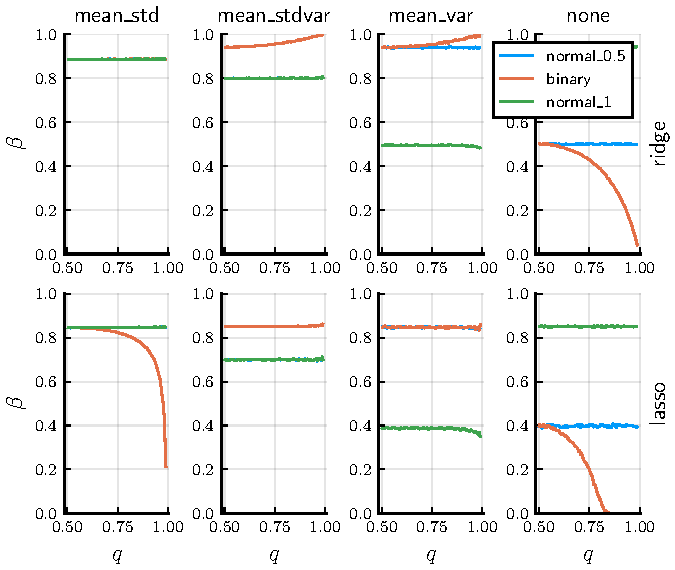
\includegraphics[]{plots/lasso_ridge_twodim.pdf}
  \caption{%
    Comparison between lasso and ridge estimators for a two-dimensional problem where one feature is generated from \(\bernoulli(q)\) and the other from \(\normal(0, 0.5)\). The ridge estimator is unaffected by \(q\), but the lasso estimator is not.
  }
  \label{fig:lasso-ridge-comparison}
\end{figure}

\begin{figure}[htpb]
  \centering
  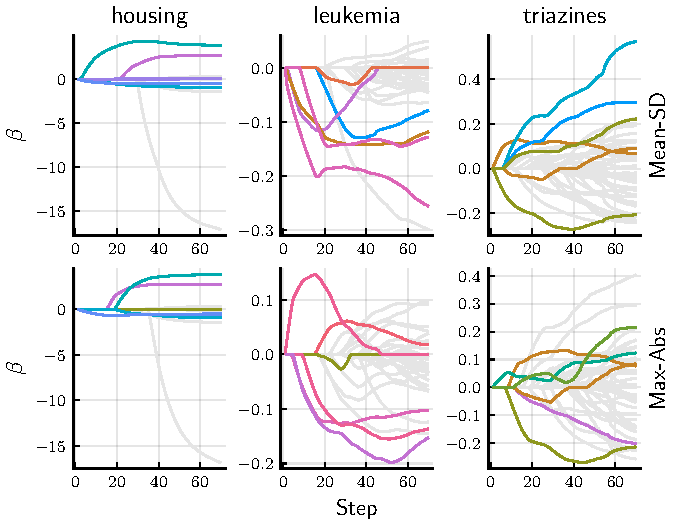
\includegraphics[]{plots/realdata_paths.pdf}
  \caption{%
    A display over the first predictors selected by the lasso for each type of normalization. Each panel shows the union of the first five predictors picked by either type of normalization.
  }
  \label{fig:realdata-paths}
\end{figure}

\subsection{Maximum Absolute Value Scaling}

In \Cref{fig:maxabs-n} we show how the coefficient corresponding to the Normally distributed feature shrinks as the number of observation \(n\) increases.

\begin{figure}[htpb]
  \centering
  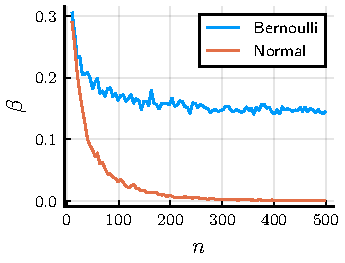
\includegraphics[]{plots/maxabs_n.pdf}
  \caption{%
    Effects of maximum absolute value scaling.
  }
  \label{fig:maxabs-n}
\end{figure}

\printbibliography

\end{document}
